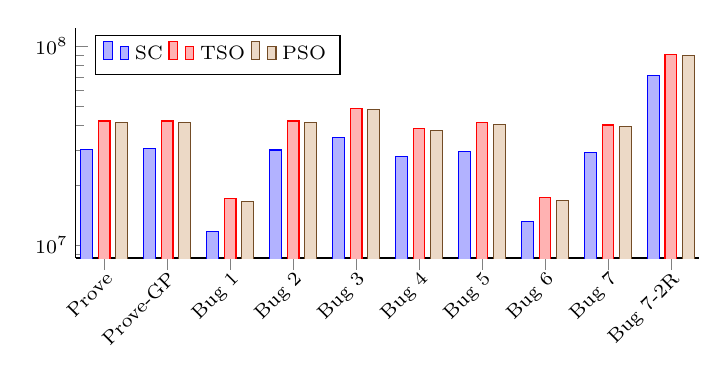
\begin{tikzpicture}
\scriptsize
\begin{axis}[
  ybar,
  bar width=0.15cm,
  height=4.5cm,
  width=9.5cm,
  axis lines*=left, % remove lines in the background
  ymode=log,
  %ylabel=Number of variables,
  symbolic x coords={Prove, Prove-GP, Bug 1, Bug 2, Bug 3, 
                     Bug 4, Bug 5, Bug 6, Bug 7, Bug 7-2R,
                    },
  xtick=data,
  %nodes near coords, % numbers displayed above the bars
  %every node near coord/.append style={font=\small, rotate=90, anchor=west},
  xticklabel style={
    inner sep=0pt,
    anchor=north east,
    rotate=45
  },
  %enlargelimits=0.15,
  enlarge y limits=0.15, % space relative to the height of the plot
  enlarge x limits=0.05, % space relative to the width of the plot
  legend style={
    %anchor=north, at={(0.5, -0.9)}, % legend location
    legend pos=north west,
    legend columns=-1,
    font=\scriptsize},
]

\addplot % SC
  coordinates {(Prove, 30085337) (Prove-GP, 30655428)
               (Bug 1, 11719966) (Bug 2, 30056615) (Bug 3, 34856577)
               (Bug 4, 27804363) (Bug 5, 29510828) (Bug 6, 13165176)
               (Bug 7, 29242760) (Bug 7-2R, 71205400)
              };

\addplot % TSO 
  coordinates {(Prove, 42042386) (Prove-GP, 42041740)
               (Bug 1, 17120555) (Bug 2, 42013372) (Bug 3, 48788433)
               (Bug 4, 38480891) (Bug 5, 41239083) (Bug 6, 17286058)
               (Bug 7, 40139251) (Bug 7-2R, 90444903)
              };


\addplot % PSO
  coordinates {(Prove, 41327066) (Prove-GP, 41326420)
               (Bug 1, 16548819) (Bug 2, 41298052) (Bug 3, 48023601)
               (Bug 4, 37765571) (Bug 5, 40529619) (Bug 6, 16766198)
               (Bug 7, 39442675) (Bug 7-2R, 89398551)
              };

\legend{SC, TSO, PSO}
\end{axis}
\end{tikzpicture}
